\documentclass[notes,11pt, aspectratio=169]{beamer}

\usepackage{pgfpages}
\setbeameroption{hide notes} % Only slide

\usepackage{array}
\usepackage{tikz}
\usepackage{verbatim}
\setbeamertemplate{note page}{\pagecolor{gray!5}\insertnote}
\usetikzlibrary{positioning}
\usetikzlibrary{snakes}
\usetikzlibrary{calc}
\usetikzlibrary{arrows}
\usetikzlibrary{decorations.markings}
\usetikzlibrary{shapes.misc}
\usetikzlibrary{matrix,shapes,arrows,fit,tikzmark}
\usepackage{amsmath}
\usepackage{mathpazo}
\usepackage{hyperref}
\usepackage{lipsum}
\usepackage{multimedia}
\usepackage{graphicx}
\usepackage{multirow}
\usepackage{dcolumn}
\usepackage{bbm}
\newcolumntype{d}[0]{D{.}{.}{5}}

\usepackage{changepage}
\usepackage{appendixnumberbeamer}
\newcommand{\beginbackup}{
   \newcounter{framenumbervorappendix}
   \setcounter{framenumbervorappendix}{\value{framenumber}}
   \setbeamertemplate{footline}
   {
     \leavevmode%
     \hline
     box{%
       \begin{beamercolorbox}[wd=\paperwidth,ht=2.25ex,dp=1ex,right]{footlinecolor}%
       \end{beamercolorbox}}%
     \vskip0pt%
   }
 }
\newcommand{\backupend}{
   \addtocounter{framenumbervorappendix}{-\value{framenumber}}
   \addtocounter{framenumber}{\value{framenumbervorappendix}}
}

\usepackage[space]{grffile}
\usepackage{booktabs}

% Colors
\definecolor{blue}{RGB}{0,114,178}
\definecolor{red}{RGB}{213,94,0}
\definecolor{yellow}{RGB}{240,228,66}
\definecolor{green}{RGB}{0,158,115}

\hypersetup{
  colorlinks=false,
  linkbordercolor = {white},
  linkcolor = {blue}
}

\definecolor{MyBackground}{RGB}{255,253,218}

\newenvironment{transitionframe}{
  \setbeamercolor{background canvas}{bg=white}
  \begin{frame}}{
    \end{frame}
}

\setbeamercolor{frametitle}{fg=blue}
\setbeamercolor{title}{fg=black}
\setbeamertemplate{footline}[frame number]
\setbeamertemplate{navigation symbols}{}
\setbeamertemplate{itemize items}{-}
\setbeamercolor{itemize item}{fg=blue}
\setbeamercolor{itemize subitem}{fg=blue}
\setbeamercolor{enumerate item}{fg=blue}
\setbeamercolor{enumerate subitem}{fg=blue}
\setbeamercolor{button}{bg=MyBackground,fg=blue,}

\setbeamercolor{section in toc}{fg=blue}
\setbeamercolor{subsection in toc}{fg=red}
\setbeamersize{text margin left=1em,text margin right=1em}

\newenvironment{wideitemize}{\itemize\addtolength{\itemsep}{10pt}}{\enditemize}
\newenvironment{wideenumerate}{\enumerate\addtolength{\itemsep}{10pt}}{\endenumerate}

%%% TIKZ STUFF
\tikzset{
        every picture/.style={remember picture,baseline},
        every node/.style={anchor=base,align=center,outer sep=1.5pt},
        every path/.style={thick},
        }
\newcommand\marktopleft[1]{%
    \tikz[overlay,remember picture]
        \node (marker-#1-a) at (-.3em,.3em) {};%
}
\newcommand\markbottomright[2]{%
    \tikz[overlay,remember picture]
        \node (marker-#1-b) at (0em,0em) {};%
}
\tikzstyle{every picture}+=[remember picture]
\tikzstyle{mybox} =[draw=black, very thick, rectangle, inner sep=10pt, inner ysep=20pt]
\tikzstyle{fancytitle} =[draw=black,fill=red, text=white]
%%%% END TIKZ STUFF

\title[]{\textcolor{blue}{ECN 594: Logit Demand and Identification}}
\author[PGP]{}
\institute[FRBNY]{\small{\begin{tabular}{c c c}
Nicholas Vreugdenhil \\
\end{tabular}}}
\date{\today}

\begin{document}

% Title Slide
\begin{frame}
\maketitle
  \centering
\end{frame}

\begin{frame}{Announcements}
	\begin{wideitemize}
		\item \textbf{Homework 1 released today}
		\item Due: Feb 4 (before Lecture 6)
		\item Demand estimation using Python and \texttt{pyblp}
		\item Start early!
	\end{wideitemize}
\end{frame}

\begin{frame}{Plan for today}
  \begin{wideenumerate}
    \item Logit model derivation
    \item Berry (1994) inversion
    \item Elasticity formulas
    \item IIA problem (preview)
    \item[] \rule{0.5\textwidth}{0.4pt}
    \item The identification problem
    \item Direction of bias
    \item Instrumental variables
    \item Uber example
  \end{wideenumerate}
\end{frame}

%%%%%%%%%%%%%%%%%%%%%%%%%%%%%%%%%%%%%%%%%%%%%%%%%%%%%%%%%%%%%
% PART 1: LOGIT DEMAND MODEL
%%%%%%%%%%%%%%%%%%%%%%%%%%%%%%%%%%%%%%%%%%%%%%%%%%%%%%%%%%%%%

\begin{transitionframe}
	\begin{center}
		{\Huge Part 1: The Logit Demand Model}
	\end{center}
\end{transitionframe}

\begin{frame}{Recap: Random utility}
	\begin{wideitemize}
		\item Consumer $i$ chooses among $J$ products
		\item Utility:
		\begin{align*}
			u_{ij} = x_j \beta - \alpha p_j + \xi_j + \varepsilon_{ij}
		\end{align*}
		\item Consumer chooses the product with highest utility
		\item Last time: we left $\varepsilon_{ij}$ unspecified
		\item Today: we assume $\varepsilon_{ij}$ has a specific distribution
	\end{wideitemize}
\end{frame}

\begin{frame}{The logit assumption}
	\begin{wideitemize}
		\item Assume $\varepsilon_{ij}$ is i.i.d. \textbf{Type I Extreme Value}
		\item Also called Gumbel distribution
		\item CDF: $F(\varepsilon) = \exp(-\exp(-\varepsilon))$
		\item Why this assumption?
		\begin{wideitemize}
			\vspace{5pt}
			\item Gives us \textbf{closed-form} choice probabilities!
			\item Computationally tractable
		\end{wideitemize}
	\end{wideitemize}
\end{frame}

\begin{frame}{Logit choice probabilities}
	\begin{wideitemize}
		\item Define \textbf{mean utility}:
		\begin{align*}
			\delta_j = x_j \beta - \alpha p_j + \xi_j
		\end{align*}
		\item So utility is: $u_{ij} = \delta_j + \varepsilon_{ij}$
		\item With Type I Extreme Value errors, the probability that consumer chooses $j$:
		\begin{align*}
			P(\text{choose } j) = \frac{\exp(\delta_j)}{\sum_{k=1}^J \exp(\delta_k)}
		\end{align*}
		\item This is the \textbf{logit} formula
	\end{wideitemize}
\end{frame}

\begin{frame}{The outside option}
	\begin{wideitemize}
		\item Problem: Our formula doesn't allow consumers to ``not buy''
		\item We need an \textbf{outside option} (product $j=0$)
		\item Utility of outside option:
		\begin{align*}
			u_{i0} = \varepsilon_{i0}
		\end{align*}
		\item We normalize: $\delta_0 = 0$
		\item All other utilities are \textit{relative} to this outside option
	\end{wideitemize}
\end{frame}

\begin{frame}{Logit with outside option}
	\begin{wideitemize}
		\item With the outside option, the share of product $j$ is:
		\begin{align*}
			s_j = \frac{\exp(\delta_j)}{1 + \sum_{k=1}^J \exp(\delta_k)}
		\end{align*}
		\item And the share of the outside option is:
		\begin{align*}
			s_0 = \frac{1}{1 + \sum_{k=1}^J \exp(\delta_k)}
		\end{align*}
		\item Note: $s_0 + \sum_{j=1}^J s_j = 1$ (shares sum to 1)
	\end{wideitemize}
\end{frame}

\begin{frame}{Berry (1994) inversion: the key insight}
	\begin{wideitemize}
		\item We observe: market shares $s_j$
		\item We want: mean utilities $\delta_j$ (to estimate $\beta$, $\alpha$)
		\item \textbf{Problem:} How do we get $\delta_j$ from $s_j$?
		\item \textbf{Berry's insight:} Take the log of shares!
	\end{wideitemize}
\end{frame}

\begin{frame}{Berry (1994) inversion}
	\begin{wideitemize}
		\item Start with:
		\begin{align*}
			s_j = \frac{\exp(\delta_j)}{1 + \sum_{k=1}^J \exp(\delta_k)}, \quad s_0 = \frac{1}{1 + \sum_{k=1}^J \exp(\delta_k)}
		\end{align*}
		\item Take logs:
		\begin{align*}
			\ln(s_j) &= \delta_j - \ln\left(1 + \sum_{k=1}^J \exp(\delta_k)\right) \\
			\ln(s_0) &= -\ln\left(1 + \sum_{k=1}^J \exp(\delta_k)\right)
		\end{align*}
		\item Subtract:
		\begin{align*}
			\ln(s_j) - \ln(s_0) = \delta_j
		\end{align*}
	\end{wideitemize}
\end{frame}

\begin{frame}{Berry (1994) inversion: the estimating equation}
	\begin{wideitemize}
		\item We have: $\ln(s_j) - \ln(s_0) = \delta_j$
		\item Substitute $\delta_j = x_j \beta - \alpha p_j + \xi_j$:
		\begin{align*}
			\ln(s_j) - \ln(s_0) = x_j \beta - \alpha p_j + \xi_j
		\end{align*}
		\item This is a \textbf{linear regression}!
		\item LHS: can compute from observed shares
		\item RHS: product characteristics, price, and an error term
	\end{wideitemize}
\end{frame}

\begin{frame}{Logit elasticities}
	\begin{wideitemize}
		\item Given shares $s_j = \frac{\exp(\delta_j)}{1 + \sum_k \exp(\delta_k)}$
		\item We can derive price elasticities:
		\begin{align*}
			\eta_{jj} &= \frac{\partial s_j}{\partial p_j} \frac{p_j}{s_j} = -\alpha p_j (1 - s_j) \quad \text{(own-price)} \\[10pt]
			\eta_{jk} &= \frac{\partial s_j}{\partial p_k} \frac{p_k}{s_j} = \alpha p_k s_k \quad \text{(cross-price)}
		\end{align*}
		\item Note: $\alpha > 0$, so own-price elasticity is \textbf{negative} (as expected)
	\end{wideitemize}
\end{frame}

\begin{frame}{Worked example: Logit elasticities}
	\begin{wideitemize}
		\item \textbf{Question:}
		\item Suppose $\alpha = 0.5$, product $j$ has price $p_j = 20$ and market share $s_j = 0.1$.
		\item Compute the own-price elasticity for product $j$.
	\end{wideitemize}
	\vspace{20pt}
	\centering
	\textit{Take 2 minutes to solve this.}
\end{frame}

\begin{frame}{Worked example: Logit elasticities (solution)}
	\begin{wideitemize}
		\item Own-price elasticity formula:
		\begin{align*}
			\eta_{jj} = -\alpha p_j (1 - s_j)
		\end{align*}
		\item Plug in: $\alpha = 0.5$, $p_j = 20$, $s_j = 0.1$
		\begin{align*}
			\eta_{jj} &= -0.5 \times 20 \times (1 - 0.1) \\
			&= -0.5 \times 20 \times 0.9 \\
			&= -9
		\end{align*}
		\item Interpretation: A 1\% price increase $\Rightarrow$ 9\% decrease in quantity
	\end{wideitemize}
\end{frame}

\begin{frame}{Worked example: Cross-price elasticity}
	\begin{wideitemize}
		\item Now compute the cross-price elasticity with product $k$
		\item Given: $\alpha = 0.5$, $p_k = 25$, $s_k = 0.05$
		\item Cross-price elasticity formula:
		\begin{align*}
			\eta_{jk} = \alpha p_k s_k
		\end{align*}
		\item Plug in:
		\begin{align*}
			\eta_{jk} &= 0.5 \times 25 \times 0.05 \\
			&= 0.625
		\end{align*}
		\item Interpretation: A 1\% increase in $p_k$ $\Rightarrow$ 0.625\% increase in $s_j$
	\end{wideitemize}
\end{frame}

\begin{frame}{The IIA problem (preview)}
	\begin{wideitemize}
		\item Look at the cross-price elasticity again:
		\begin{align*}
			\eta_{jk} = \alpha p_k s_k
		\end{align*}
		\item This doesn't depend on product $j$ at all!
		\item Implication: All products have the \textbf{same} cross-elasticity with product $k$
		\item Is this realistic?
		\item Suppose BMW raises its price. Logit says: same fraction go to Mercedes as to Honda Civic!
		\item This is the \textbf{IIA} (Independence of Irrelevant Alternatives) property
		\item We'll discuss this in detail in Lecture 4
	\end{wideitemize}
\end{frame}

%%%%%%%%%%%%%%%%%%%%%%%%%%%%%%%%%%%%%%%%%%%%%%%%%%%%%%%%%%%%%
% PART 2: IDENTIFICATION AND IVs
%%%%%%%%%%%%%%%%%%%%%%%%%%%%%%%%%%%%%%%%%%%%%%%%%%%%%%%%%%%%%

\begin{transitionframe}
	\begin{center}
		{\Huge Part 2: Identification and Instrumental Variables}
	\end{center}
\end{transitionframe}

\begin{frame}{The estimating equation (reminder)}
	\begin{wideitemize}
		\item From Berry inversion:
		\begin{align*}
			\ln(s_j) - \ln(s_0) = x_j \beta - \alpha p_j + \xi_j
		\end{align*}
		\item This looks like a regression we can run with OLS
		\item \textbf{But there's a problem...}
	\end{wideitemize}
\end{frame}

\begin{frame}{The classic identification problem}
	\begin{wideitemize}
		\item We observe equilibrium prices and quantities
		\item Problem: can't tell if demand shifted or supply shifted
	\end{wideitemize}
	\begin{figure}
		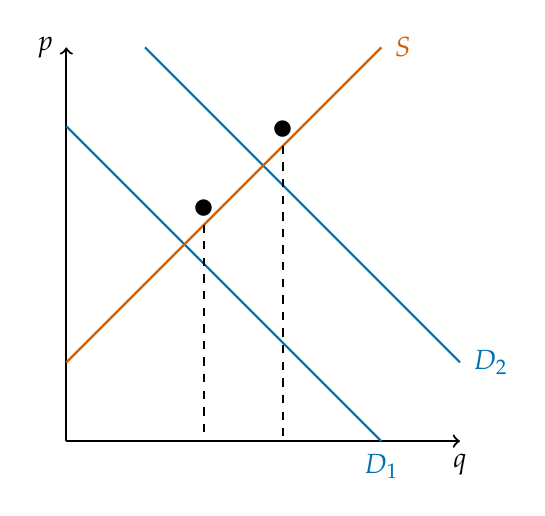
\begin{tikzpicture}[scale=0.5]
			%y axis
			\draw [->] (0,0) to (0,10) node [left] {$p$};
			%x axis
			\draw [->] (0,0) to (10,0) node [below] {$q$};

			% D curves
			\draw [thick, blue] (0,8) to (8,0) node [below] {$D_1$};
			\draw [thick, blue] (2,10) to (10,2) node [right] {$D_2$};

			% S curve
			\draw [thick, red] (0,2) to (8,10) node [right] {$S$};

			% equilibrium points
			\node [black] at (3.5,5.5) {\LARGE \textbullet};
			\node [black] at (5.5,7.5) {\LARGE \textbullet};

			\draw [dashed] (3.5,5.5) to (3.5,0);
			\draw [dashed] (5.5,7.5) to (5.5,0);
		\end{tikzpicture}
	\end{figure}
\end{frame}

\begin{frame}{The classic identification problem}
	\begin{wideitemize}
		\item If we just regress $q$ on $p$, what do we get?
		\item Neither demand nor supply!
		\item \textbf{Key insight:} We need variation that shifts ONE curve but not the other
		\begin{wideitemize}
			\vspace{5pt}
			\item To identify demand: need \textbf{supply shifters}
			\item To identify supply: need \textbf{demand shifters}
		\end{wideitemize}
	\end{wideitemize}
\end{frame}

\begin{frame}{Price endogeneity in demand estimation}
	\begin{wideitemize}
		\item Our estimating equation:
		\begin{align*}
			\ln(s_j) - \ln(s_0) = x_j \beta - \alpha p_j + \xi_j
		\end{align*}
		\item $\xi_j$ = unobserved product quality
		\item \textbf{Problem:} Firms observe $\xi_j$ when setting prices!
		\item High quality products ($\xi_j$ high) tend to have high prices
		\item $\Rightarrow$ $\text{Cov}(p_j, \xi_j) > 0$
		\item OLS gives biased estimates
	\end{wideitemize}
\end{frame}

\begin{frame}{Direction of bias}
	\begin{wideitemize}
		\item If high-quality products have high prices...
		\item OLS sees: high price, but demand still high (because of $\xi$)
		\item OLS concludes: price doesn't hurt demand much
		\item \textbf{Result:} $\hat{\alpha}$ biased toward zero (less negative than truth)
	\end{wideitemize}
\end{frame}

\begin{frame}{Worked example: Bias direction}
	\begin{wideitemize}
		\item \textbf{Question:} You estimate a logit demand model using OLS and get $\hat{\alpha} = -0.3$. A colleague says the true $\alpha$ is likely $-0.5$.
		\item Is this consistent with endogeneity bias? Why?
		\pause
		\item \textbf{Answer:} Yes!
		\begin{wideitemize}
			\vspace{5pt}
			\item OLS overstates how much consumers like expensive products
			\item So OLS finds a smaller (less negative) price coefficient
			\item $-0.3 > -0.5$, so this is exactly what we'd expect
		\end{wideitemize}
	\end{wideitemize}
\end{frame}

\begin{frame}{The gold standard: Experiments}
	\begin{wideitemize}
		\item Best solution: randomize prices!
		\item \textbf{Uber's price ``wiggles''} (Cohen et al. 2016)
		\begin{wideitemize}
			\vspace{5pt}
			\item Uber experimentally varies surge multipliers up and down
			\item Same time, same location $\rightarrow$ different riders see different prices
			\item This randomization creates exogenous price variation
		\end{wideitemize}
		\item Key insight: demand conditions are identical, only price differs
		\item Result: demand elasticity $\approx -0.5$ (inelastic!)
	\end{wideitemize}
\end{frame}

\begin{frame}{Why experiments are powerful}
	\begin{wideitemize}
		\item No confounding: price variation is independent of demand shocks
		\item Clean identification of the demand curve
		\item \textbf{But:}
		\begin{wideitemize}
			\vspace{5pt}
			\item Tech companies can run experiments
			\item Traditional industries can't randomize prices
			\item Most IO settings require \textbf{instrumental variables}
		\end{wideitemize}
	\end{wideitemize}
\end{frame}

\begin{frame}{Instrumental variables: the solution}
	\begin{wideitemize}
		\item Need variables $z$ that are:
		\begin{wideenumerate}
			\vspace{5pt}
			\item \textbf{Relevant:} Correlated with price ($\text{Cov}(z, p) \neq 0$)
			\item \textbf{Exogenous:} Uncorrelated with $\xi$ ($\text{Cov}(z, \xi) = 0$)
		\end{wideenumerate}
		\item These are cost shifters or other supply-side variables
	\end{wideitemize}
\end{frame}

\begin{frame}{Common IVs in demand estimation}
	\begin{wideenumerate}
		\item \textbf{Hausman IVs:} Prices in other markets
		\begin{wideitemize}
			\vspace{3pt}
			\item Same product in different cities has similar costs
			\item But demand shocks may differ across markets
		\end{wideitemize}
		\item \textbf{BLP IVs:} Characteristics of competing products
		\begin{wideitemize}
			\vspace{3pt}
			\item More/different competitors $\rightarrow$ lower prices
			\item Competitors' characteristics don't affect YOUR $\xi$
		\end{wideitemize}
		\item \textbf{Cost shifters:} Input prices, exchange rates
		\begin{wideitemize}
			\vspace{3pt}
			\item Affect production costs, hence prices
			\item No direct effect on demand
		\end{wideitemize}
	\end{wideenumerate}
\end{frame}

\begin{frame}{Worked example: IV intuition}
	\begin{wideitemize}
		\item \textbf{Question:} Why do competitor characteristics work as IVs?
		\pause
		\item \textbf{Answer:}
		\item \textbf{Relevance:} More competitors nearby $\rightarrow$ more competition $\rightarrow$ lower price $\checkmark$
		\item \textbf{Exogeneity:} Competitor characteristics don't affect YOUR unobserved quality $\xi_j$ $\checkmark$
		\item Example: If Toyota enters with a new Camry, this affects Civic's price but not Civic's unobserved quality
	\end{wideitemize}
\end{frame}

\begin{frame}{Worked example: Evaluating an IV}
	\begin{wideitemize}
		\item \textbf{Question:} A researcher proposes using gasoline prices as an IV for car prices. Is this valid?
		\pause
		\item \textbf{Relevance:} Higher gas prices $\rightarrow$ higher operating costs $\rightarrow$ might affect car prices? Maybe weakly.
		\item \textbf{Exogeneity:} Do gas prices affect car quality $\xi_j$?
		\begin{wideitemize}
			\vspace{3pt}
			\item Gas prices affect \textit{demand} for fuel-efficient cars
			\item This might shift which cars look ``good'' to consumers
			\item Potentially problematic!
		\end{wideitemize}
		\item \textbf{Verdict:} Probably not a great IV
	\end{wideitemize}
\end{frame}

\begin{frame}{Summary: IV conditions}
	\begin{wideitemize}
		\item For $z$ to be a valid IV:
		\begin{wideenumerate}
			\vspace{5pt}
			\item \textbf{Relevant:} $z$ must predict prices
			\begin{wideitemize}
				\item Can test this! Run first-stage regression
			\end{wideitemize}
			\item \textbf{Exogenous:} $z$ must not affect demand directly
			\begin{wideitemize}
				\item Cannot test this directly (requires economic reasoning)
			\end{wideitemize}
		\end{wideenumerate}
		\item This is the standard IV framework from econometrics
		\item Applied to demand estimation: use supply-side variation
	\end{wideitemize}
\end{frame}

%%%%%%%%%%%%%%%%%%%%%%%%%%%%%%%%%%%%%%%%%%%%%%%%%%%%%%%%%%%%%
% KEY POINTS
%%%%%%%%%%%%%%%%%%%%%%%%%%%%%%%%%%%%%%%%%%%%%%%%%%%%%%%%%%%%%

\begin{frame}{Key Points}
	\vspace{11pt}
	\begin{wideenumerate}
		\item \textbf{Logit model}: $\varepsilon_{ij}$ is Type I Extreme Value $\rightarrow$ closed-form shares
		\item \textbf{Share equation}: $s_j = \frac{\exp(\delta_j)}{1 + \sum_k \exp(\delta_k)}$
		\item \textbf{Berry inversion}: $\ln(s_j) - \ln(s_0) = \delta_j$ turns demand estimation into a regression
		\item \textbf{Elasticities}: Own $= -\alpha p_j(1-s_j)$; Cross $= \alpha p_k s_k$
		\item \textbf{IIA}: Cross-elasticities don't depend on product similarity (a limitation)
		\item \textbf{Price is endogenous}: Firms observe $\xi_j$ when pricing $\rightarrow$ $\text{Cov}(p, \xi) > 0$
		\item \textbf{Bias direction}: OLS gives $\hat{\alpha}$ biased toward zero
		\item \textbf{Solution}: Instrumental variables (cost shifters, BLP IVs, Hausman IVs)
	\end{wideenumerate}
\end{frame}

\begin{frame}{Next time}
	\begin{wideitemize}
		\item \textbf{Lecture 3:} Demographic Interactions and pyblp
		\begin{wideitemize}
			\vspace{5pt}
			\item Extending logit to allow preference heterogeneity
			\item Estimation using pyblp package
			\item Worked example with car data
		\end{wideitemize}
	\end{wideitemize}
\end{frame}

\end{document}
